\documentclass[12pt,a4paper,final]{article}
\usepackage[utf8]{inputenc}
\usepackage[T1]{fontenc}
\usepackage{amsmath}
\usepackage{amssymb}
\usepackage{graphicx}
\usepackage[left=3.00cm, right=2.50cm, top=2.50cm, bottom=2.50cm]{geometry}
\usepackage[spanish]{babel}
\usepackage{setspace}
\usepackage{titlesec}
\pagestyle{plain}
\usepackage{pgfgantt}
\usepackage{lscape}
\usepackage{float}

\usepackage[backend=bibtex,style=authoryear]{biblatex}
\addbibresource{citasArmadillo.bib}

%interlineado 
\spacing{1.5}
%espacio entre parrafos
\setlength{\parskip}{2mm}
%sangria
\setlength{\parindent}{0pt}

\setcounter{secnumdepth}{4}
\setcounter{tocdepth}{4}

\newcommand\caratuladc{\fontsize{15pt}{15pt}\selectfont}
\newcommand\titulodc{\fontsize{16pt}{16pt}\selectfont}
\newcommand\titulosndc{\fontsize{14pt}{14pt}\selectfont}
\newcommand\titulotndc{\fontsize{12pt}{12pt}\selectfont}

\titleformat*{\section}{\titulotndc \bfseries}
\titleformat*{\subsection}{\titulotndc \bfseries}
\titleformat*{\subsubsection}{\titulotndc \bfseries}

% Useful packages
\usepackage{amsmath}
\usepackage{graphicx}
\graphicspath{{images/}}
\usepackage[colorlinks=true, allcolors=blue]{hyperref}

\begin{document}
	
	\section{TITULO}
	
	\par{LIBRERÍA JAVASCRIPT PARA INTERPRETAR LA ESCRITURA DE LOS CASOS DE USO EXTENDIDOS USANDO UN LENGUAJE DE SÍMBOLOS}
	
	\section{INTRODUCCIÓN}
	
	El desarrollo de software se vuelve cada vez más indispensable en todos los aspectos de la vida cotidiana, por lo cual se necesitan herramientas que ayuden a agilizar la construcción de diferentes tipos de sistemas de información basados en computadoras (SI) \cite{DeLone}. Utilizando el Lenguaje unificado de modelado (Unified Modeling Language: UML), se pretenden utilizar el diagrama de clases como elemento principal para identificar de manera sencilla como interactuarán todos los objetos del sistema \cite{UMLsequence}. El uso de diagrama de clases constituye una buena solución del modelado de SI, en especial, aquellos proyectos en dónde los requisitos están cambiando constantemente \cite{review}, por lo que necesario una herramienta que permita la actualización de sus modelos con el menor de los esfuerzos.
	
	\section{PROBLEMATIZACIÓN}
	
	El mayor enigma en el desarrollo de un software surge al diseñar su estructura principal por no conocer totalmente la lógica de negocio que se va a automatizar \cite{Weighted}.  Para disminuir el impacto de esta problemática se sugiere el uso de diagramas de clases, es decir que a través de las entidades, sus atributos y métodos facilita las tareas de los diseñadores informáticos y también reduce las tareas de diseño del software \cite{Management}.
	
	Para construir un diagrama de clases se deben manipular herramientas que permitan crear cada componente, con pocos conocimientos sobre cada objeto que interviene en la construcción del mismo \cite{Management}. Además, al momento de continuar con el desarrollo del sistema surgirán modificaciones en requisitos que ya fueron planteados al inicio del proyecto, lo cual provoca malestar en los desarrolladores, ya que; se debe editar los objetos del diagrama sin tener algún tipo de información que permita recordar lo que ya estaba desarrollado \cite{case}.
	
	Para obtener información que ya fue analizada sobre le diagrama de clases que se tenga creado, se pretende utilizar un lenguaje simbólico que se encuentra en la herramienta TDDTIoTS (https://aplicaciones.uteq.edu.ec/tddt4iots), este lenguaje no notifica mensajes de advertencia sobre el estado de los textos que describen los casos de uso, además se necesita una documentación más detallada sobre cómo utilizar cada símbolo al momento de describir las acciones de cada caso de uso y no tener inconvenientes al tratar de interpretar cada párrafo. En definitiva, existen varios inconvenientes para crear un diagrama de clases que permita identificar de forma sencilla todo el proceso que se quiere realizar con e software, provocando malos entendidos al momento de empezar a desarrollar el código del sistema.
	
	\section{JUSTIFICACIÓN}
	La construcción de los diagramas de clases tienden a contener información redundante o aveces inconsistente para especificar de forma técnica los requisitos funcionales y no funcionales de un sistema informático. Debido a esto se propone el desarrollo de una librería JavaScript, que mediante el lenguaje de símbolos usado por la herramienta TDDT4IoTs para interpretar las descripciones de los casos de uso extendidos, permitan generar de forma automática el diagrama de clases pertinente a los casos de uso planteados. 
	
	Ademas esta librería propone generar 2 tipos de estructuras que son JSON y XML que son usadas a nivel global por varias tecnologías de desarrollo, permitiendo combinar el uso de la estructura generada por esta herramienta con las librerías externas dedicadas a la creación de diferentes tipos de diagramas, obteniendo como resultado una grafico visual en relación a la información devuelta por el producto final de este proyecto. 
	
	\section{FORMULACIÓN}
	
	¿Como interpretar las descripciones de los casos de uso extendidos escritos en el lenguaje de símbolos usado en la herramienta TDDT4IoTS para generar la estructura de un diagrama de clases?
	
	\subsection{Sistematización}
	
	\begin{enumerate}
		\item ¿Como se obtendrá el diagrama de clases generado por las descripciones de los casos de uso extendidos?
		
		\item ¿Como ayudar a los usuarios a mejorar la escritura de las descripciones de los casos de uso extendidos escritos en un lenguaje de símbolos usado por la herramienta TDDT4IoTS?
		
		\item ¿De que forma se evaluara el correcto funcionamiento del producto final de este proyecto de investigación?
	\end{enumerate}
	
	\section{OBJETIVOS}
	
	La problematización de este proyecto ha llevado a plantearse los siguiente objetivos.
	
	\subsection{Objetivo principal}
	
	Desarrollar una librería JavaScript que interprete las descripciones de los casos de uso usado la herramienta TDDT4IoTS para visualizar la estructura del diagrama de clases pertinente. 
	
	\subsection{Objetivos específicos}
	
	\begin{enumerate}
		\item Generar una estructura JSON y XML con la información obtenida por las descripciones de los casos de uso extendidos para crear un diagrama de clases mediante el uso librerías javascript para crear diagramas.
		
		\item Retroalimentar a los usuarios sobre la mala escritura de las descripciones de los casos de uso extendidos escritos en un lenguaje de símbolos usado por la herramienta TDDT4IoTSs. 
		
		\item Evaluar la librería JavaScript con la elaboración de diagramas de clases a partir de casos de uso extendidos correspondientes a sistemas de información reales.
	\end{enumerate}
	
	
	\section{ESQUEMA REFERENCIAL DEL MARCO TEÓRICO}
	
	En este capítulo, se expondrán los trabajos relacionados con el presentado en este documento que se han identificado en la literatura, y que demuestran que el trabajo propuesto en este documento, aporta algo. Además se contextualiza el trabajo y define los términos novedosos y de poco dominio para los investigadores y para la comunidad.
	
	\subsection{Marco Referencial}
	
	\textbf{Lenguaje de restricciones de objetos para la generación de código
	a partir de modelos de actividad.} UML(Unified Modeling Language) es un lenguaje que utiliza el diagrama de actividad para modelar el flujo de trabajo y el flujo de objetos en un sistema \cite{Improving}. UML no es un lenguaje totalmente formal, su semántica no está totalmente formalizada ocasionando un escenario donde la presentación precisa del modelo es difícil. Por lo tanto, siempre que se utilicen diagramas de actividades, o cualquier diagrama UML, para la generación de código, se recomienda complementarlo con lenguajes de especificación como el lenguaje de restricciones de objetos OCL (Object Constraint Language) \cite{Object}.   

	\textbf{Desarrollo de módulos de software generativo para el diseño orientado al dominio con un lenguaje específico de dominio basado en anotaciones. }En la terminología del diseño orientado a objetos \cite{Feature}, un módulo de dominio es un paquete. Los actuales marcos de software DDD (Object-oriented domain-driven design) han utilizando una forma simple de DSL(Domain-specific language) interno para construir el modelo de dominio y utilizar este modelo como entrada para generar un prototipo de software. El DSL interno que utilizan se conoce más formalmente como lenguaje específico del dominio basado en anotaciones (aDSL) \cite{Generative}. 
	
	\textbf{Modelado para la localización de características en modelos de software: tanto la generación de código y los modelos interpretados. }Evaluando LDA (Latent Dirichlet Allocation), cada caso de estudio utiliza un tipo diferente de modelos de software: modelos de software para la generación de código, y modelos de software para interpretación. El primer caso de estudio pertenece a un líder mundial en fabricación de trenes, construcciones y Auxiliar de Ferrocarriles. Una empresa que formaliza los productos fabricados en modelos de software utilizando un lenguaje específico de dominio DSL. Los modelos de software se utilizan para generar el firmware que controla sus trenes \cite{Topic}. 
	
	El segundo estudio de caso pertenece a un videojuego comercial, Kromaia, que utiliza modelos de software para razonar sobre el sistema, realizar validaciones y definir el contenido del juego, como los jefes, los mundos y los objetivos. En Kromaia los modelos de software se utilizan para la interpretación. Así, el contenido definido en los modelos se lee e interpreta cuando se lanza el juego (sin alterar el código fuente del videojuego). El videojuego se ha lanzado en todo el mundo en dos plataformas diferentes (PlayStation 4 y STEAM) y en 8 idiomas diferentes. \cite{Topic}.
	
	\subsection{Marco Contextual}
	
	En esta sección, se describe el entorno de trabajo investigativo realizado a este proyecto. Este marco complementa al resto de los referentes, que sirven de marco a una investigación.
		
	\subsubsection{Metodología ágil}
	
	Esta metodología consta de 5 fases. Aparentemente agrupan fases que estén relacionadas al desarrollo de un sistema, desde el análisis de requisitos hasta su debido mantenimiento. Esta última es muy olvidada por los investigadores, y es de mucho interés en la vida de desarrollo. En la figura \ref{fig:metod} se pueden observar las fases que se deberían implementar.
	
	\begin{figure}[h!]
		\centering
		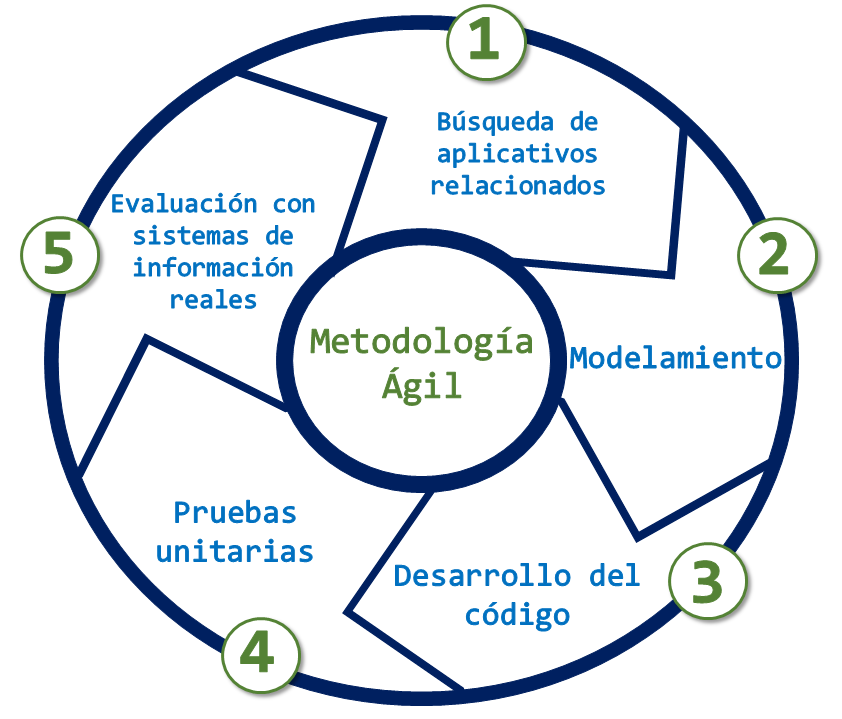
\includegraphics[width=10cm]{images/metodologia.png}
		\caption{Fases de la metodología.}
		\label{fig:metod}
	\end{figure}
	
	\paragraph{Descripción general de la metodología}
	Las principales razones del uso de una metodología ágil es el uso de un ciclo de desarrollo iterativo e incremental para la ejecución de este proyecto son:
	
	\begin{itemize}
		\item Entregas frecuentes y continuas de forma que puede disponer de una funcionalidad básica en un tiempo mínimo y a partir de ahí un incremento y mejora continua del sistema.
		
		\item Previsible inestabilidad de requisitos. Es posible que el sistema incorpora más funcionalidades de las inicialmente identificadas
		
		\item Es posible que durante la ejecución del proyecto se altere el orden en el que se desean recibir los módulos.
	\end{itemize} 
	
	\paragraph{Roles}
	
	El equipo de esta metodología está conformado por 2 roles, Director de proyecto (DP) y el Desarrollador de Sistemas (DS). Todos los miembros de un equipo de desarrollo tienen diferentes roles en la gestión y supervisión de los proyectos. Todos los roles son necesarios para que el proceso funcione eficientemente. 
	
	\begin{itemize}
		\item \textbf{Director de proyecto (DP):} Se encarga de administrar el proceso del proyecto, su planificación, coordinación con el analista y realizar un seguimiento e informes del progreso del proyecto, en términos de calidad, costo y plazos de entrega. El DP es la interfaz principal entre el propietario del producto y el analista de desarrollo de software.
		
		\item \textbf{Desarrollador de Sistemas (DS):} El desarrollador hace el trabajo. Debe tener la capacidad de organizarse y completar una característica centrada en el cliente. Las principales funciones son:
		
		\begin{itemize}
			\item Comprometerse al inicio de cada modulo y desarrollar todas las funcionalidades en el tiempo determinado.
			
			\item Son responsables de entregar un producto a cada término de un modulo.
			
			\item Definir el desarrollo del sistema.
		\end{itemize} 
	\end{itemize}

	\paragraph{Fases}
	
	\begin{enumerate}
		\item \textbf{Búsqueda de aplicativos relacionados:} Buscar aplicativos que realicen procesos similares al que se esta desarrollando. Se deberán especificar varios criterios sobre sus funcionalidades, ventajas y desventajas, vulnerabilidades, versiones, etc. 
		\item \textbf{Modelamiento:} En esta sección se empezaría a realizar el análisis de requisitos funcionales y no funcionales con los que debe contar el producto final.
		\item \textbf{Desarrollo del código:} Se debe empezar con toda la programación del sistema, es decir la escritura de todo el código usando las estructuras necesarios que permitan cumplir con todos los requisitos planteados en la fase anterior. 
		\item \textbf{Pruebas unitarias:} Con todo el desarrollo del producto finalizado, se empieza una fase de pruebas unitarias. Se deben buscar los posibles escenarios a ocurrir al momento de utilizar el sistema,  verificando si la información de entrada y salida es la correcta o incorrecta. 		
		\item \textbf{Evaluación con sistemas de información reales:} Finalmente se pueden utilizar estudios de caso reales que puedan ser aplicados sobre el producto final.
	\end{enumerate}
	
	\subsection{Marco Conceptual}
	En esta sección, se detalla los modelos teóricos, conceptos, argumentos o definiciones que se han desarrollado o investigado en relación con el tema en particular.
	
	\subsubsection{JSON}
	
	Javascript Object Notation (JSON) es un formato ligero de intercambio de datos. Consisten en asociación de nombres y valores. A pesar de ser independiente del lenguaje de programación, es admitido en una gran cantidad de lenguajes de programación. Se basa en un subconjunto del Estándar de lenguaje de programación JavaScript \cite{JSON}.
	
    \subsubsection{XML}
    
    Es un lenguaje de marcado similar a HTML. Significa Extensible Markup Language y pertenece a la especificación W3C como lenguaje de marcado de propósito general. Esto significa que, a diferencia de otros lenguajes de marcado, XML no está predefinido, por lo que debe definir su propio marcado. El objetivo principal del lenguaje es compartir datos entre diferentes sistemas, como Internet \cite{XML-based}.
    
    \subsubsection{Compiladores}
    Están diseñados para traducir un fragmento de código escrito en un de lenguaje de programación a lenguaje de máquina que es, el que puede entender la computadora. El compilador analiza el código fuente en busca de errores antes de la traducción. Si se detecta un error, el compilador
    notificar al autor del código para que pueda arreglarlo.. Además, los compiladores modernos o entornos de desarrollo (IDE), puede sugerir soluciones para algunos tipos de errores usando métodos de corrección de errores \cite{CoEdit}.
    
    \subsubsection{Lenguajes de modelado}
    Representan una serie de requisitos basados en la construcción de elementos visuales para definir estructuras y comportamientos que tendrán los sistemas computarizados. UML (Lenguaje Unificado de Modelado) a través del mecanismo de perfilado, se han basado históricamente en notaciones gráficas. UML mediante el mecanismo de perfiles, maximiza la comprensión humana y facilita la comunicación entre las partes interesadas como son el cliente y desarrollador \cite{Blended}. 
    
    También existen lenguajes de modelado personalizados para distintas áreas, como por ejemplo en \cite{Multi-level} proponen un lenguaje de modelado conceptual multinivel al denominan ML2 (Lenguaje de Modelado Multinivel). El lenguaje está orientado al modelado conceptual multinivel (de dominio) y pretende cubrir un amplio conjunto de dominios multiniveles. En el diseño de ML2 sigue un enfoque basado en principios, definiendo su sintaxis abstracta para reflejar una teoría formal para el modelado multinivel que se fue desarrollado previamente.
	
	\section{METODOLOGÍA}
	
	Para el desarrollo del presente proyecto se tomarán en cuenta la ejecución de varias etapas, aplicando el Modelo de Prototipado para desarrollar un prototipo de la aplicación web que utilice el producto final de esta investigación. A continuación, se describe el enfoque metodológico correspondiente a cada una de las fases. 
	
	\subsection{Búsqueda de aplicativos relacionados}
	
	En esta fase se analizaron varias aplicaciones web que cuentan con la funcionalidad de generar diagramas de clases mediante la escritura de texto. Entre las aplicaciones analizadas se encuentran:
	
	\begin{itemize}
		\item \textbf{yuml: }Es una aplicacion web que permite crear diagramas UML mediante la escritura por comandos en texto plano. Se puede destacar que esta herramienta no permite decidir la ubicación o lugar de un elemento grafico ya que busca la mejor distribución según el diagrama generado (https://yuml.me/)
		
		\item \textbf{mermaid: }Es una herramienta de gráficos y diagramas basada en JavaScript que utiliza definiciones de texto inspiradas en Markdown y un renderizador para crear y modificar diagramas complejos. El propósito principal de Mermaid es ayudar a que la documentación se ponga al día con el desarrollo. También se destaca que la aplicación no permite modificar en tiempo real los diagramas generados (https://mermaid.live/).
		
		\item \textbf{ditaa: }Es una pequeña utilidad de línea de comandos escrita en Java, que puede convertir diagramas dibujados con arte ascii ('dibujos' que contienen caracteres que se asemejan a líneas como | / - ), en gráficos de mapa de bits adecuados. También se destaca que la aplicación no permite modificar en tiempo real los diagramas generados (http://ditaa.sourceforge.net/). 
	\end{itemize}
	
	\subsection{Modelamiento}
	
	En esta etapa se pretende modelar la funcionalidad que tendrán todos los métodos y funciones necesarias para identificar cada símbolo y poder interpretar todo el texto para generar la estructura del diagrama de clases.
	Todo el archivo JavaScript estará conformado por estructuras de datos apuntando a la programación orientada a objetos.
	
	\subsection{Desarrollo del código}
	
	La tercera etapa se dedicará al desarrollo de la librería utilizando el lenguaje de programación JavaScript. Todo el código será escrito en un solo archivo con extensión de tipo .js teniendo como ventaja poder ser vinculado dentro de cualquier archivo HTML que dese utilizar los métodos necesarios para obtener la estructura de todo el diagrama de clases en formato JSON.
	
	La estructura podrá ser utilizada por cualquier herramienta de dibujo externa que permita visualizar el diagrama de clases de la forma tradicional con todos sus componentes. A continuación, se enlista los componentes que podrán ser generados por la librería:
	
	\begin{itemize}
		\item Entidades
		\item Interfaces
		\item Enumeradores
		\item Atributos
		\item Métodos
		\item Constructores de clases
		\item Relaciones
	\end{itemize}

	\subsection{Pruebas unitarias}
	En esta fase se pretende realizar todas las pruebas posibles a las funciones que se realizaron en la fase anterior, ingresando algunos textos utilizando los símbolos esperando los valores que devuelva la librería. Algunos de los textos que serán ingresados son los siguientes:
	
	\begin{itemize}
		\item \begin{verbatim}
			Create an user *(user %.username=String, .password=String,
			.status=Status, .user type=UserType, .person=Tutor%) object
		\end{verbatim}
		
		\item \begin{verbatim}
			*(TutorDAO &id=Int [/Save/=Tutor{.tutor=Tutor}])s the tutor 
			data in the database. *¡(TutorDAO)<<*(tutor)¡
		\end{verbatim}
	
		\item \begin{verbatim}
			*(UserDAO &-id=Int [/Save/=User{.user=User}])s the user data 
			in the database. *¡(UserDAO)<<*(User)¡
		\end{verbatim}
	
		\item \begin{verbatim}
			This use case ends when the system displays the *(@Login) 
			login Interface. *¡(Login)<<*(UserDAO)¡
		\end{verbatim}
		
	\end{itemize}
	
	\subsection{Evaluación con sistemas de información reales}
	
	Se utilizaran estudios de caso con sistemas de información reales para crear las descripciones de los casos de uso extendidos de forma natural. Luego se implementaron los símbolos como se crea conveniente, dependiendo de los requisitos ingresados en el texto. Finalmente se utilizara la librería para observar como devuelve el texto nuevamente en forma natural adicional la estructura del diagrama de clases.
	
	\subsection{Modelo de prototipado}
	El Modelo de Prototipado se aplica cuando la información detallada relacionada a requerimientos de entrada y salida del sistema no está disponible. En este modelo se asume que tal vez no todos los requerimientos son conocidos en el inicio del desarrollo del sistema. Se usa generalmente cuando un sistema no existe, o en caso de un largo y complejo sistema, cuando no hay procesos manuales para determinar los requerimientos. Los pasos que se ejecutan en el modelo de prototipado son: 
	
	\begin{enumerate}
		\item \textbf{Obtención y análisis de requisitos:} es el punto de partida del modelo. El usuario es entrevistado para conocer los requisitos del sistema.
		
		\item \textbf{Diseño rápido}: teniendo claro todos los requisitos, se procede a crear un diseño rápido y preliminar incluyendo solo los aspectos más importantes 
		
		\item\textbf{ Construir el prototipo:} se trabaja con la información tomada por el diseño rápido y crear el prototipo de la aplicación.
		
		\item \textbf{Evaluación de usuarios}: el sistema es presentado a varios usuarios para evaluar y verificar sus puntos fuertes y débiles Se reciben comentarios y sugerencias que serán analizadas por los desarrolladores.
		
		\item \textbf{Reajuste del prototipo:} el prototipo actual debe reajustarse según los nuevos requerimientos, es decir que, se debe crear un nuevo prototipo con la información adicional proporcionada por los usuarios evaluados. Este nuevo prototipo será reevaluado justo como el anterior. Este proceso se repite hasta que se cumplan todos los requerimientos especificados por el usuario. Cuando el usuario esté satisfecho con el resultado, se desarrollará un sistema final basado en el prototipo final. 
		
		\item \textbf{Implementación y mantenimiento:} Una vez que se tenga listo el sistema, ya estará listo para ser desplegado a producción. El sistema se somete a un mantenimiento de rutina para minimizar el tiempo de inactividad y evitar fallas a gran escala.
		
	\end{enumerate}
	
	\newpage
	
	\begin{landscape}
	
	\section{CRONOGRAMA DE ACTIVIDADES}
	\begin{figure}[h!]
		\centering
		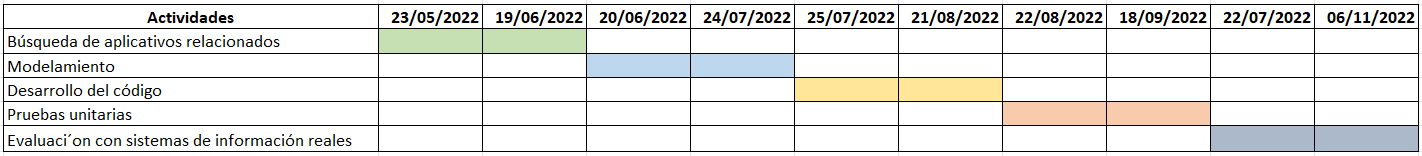
\includegraphics[width=\linewidth]{images/cronograma.png}
		\caption{Cronograma de actividades.}
		\label{fig:usecaseEasyIoT}
	\end{figure}
	
	\end{landscape}
	
	\begin{table}[!ht]
		\centering
		\begin{tabular}{|l|l|l|}
			\hline
			\multicolumn{1}{|c|}{\textbf{Fecha/actividad}}                                                                                                                                                            & \textbf{Inicio}     & \textbf{Finalización} \\ \hline
			\textbf{Búsqueda de aplicativos relacionados}                                                                                                                                                             & \textbf{23-05-2022} & \textbf{19-06-2022}   \\ \hline
			\begin{tabular}[c]{@{}l@{}}Investigar aplicaciones que cuenten con \\ funcionalidades similares al proyecto a desarrollar.\end{tabular}                                                                   & 23-05-2022          & 29-05-2022            \\ \hline
			\begin{tabular}[c]{@{}l@{}}Analizar criterios básicos de las tecnologías \\ encontradas como por ejemplo: (funcionalidades, \\ ventajas y desventajas, vulnerabilidades, \\ versiones, etc.)\end{tabular} & 31-05-2022          & 19-06-2022            \\ \hline
			\textbf{Modelamiento}                                                                                                                                                                                     & \textbf{20-06-2022} & \textbf{24-07-2022}   \\ \hline
			Análisis de los requisitos funcionales                                                                                                                                                                    & 20-06-2022          & 11-07-2022            \\ \hline
			Análisis de los requisitos no funcionales                                                                                                                                                                 & 11-07-2022          & 24-07-2022            \\ \hline
			\textbf{Desarrollo del código}                                                                                                                                                                            & \textbf{25-07-2022} & \textbf{21-08-2022}   \\ \hline
			\begin{tabular}[c]{@{}l@{}}Crear métodos y funciones que verifiquen los \\ símbolos usados por la herramienta TDDT4IoTs\end{tabular}                                                                      & 25-07-2022          & 31-07-2022            \\ \hline
			\begin{tabular}[c]{@{}l@{}}Crear la estructura JSON y XML del diagrama \\ de clases que será retornado como respuesta \\ de la librería\end{tabular}                                                      & 01-08-2022          & 21-08-2022            \\ \hline
			\textbf{Pruebas unitarias}                                                                                                                                                                                & \textbf{22-08-2022} & \textbf{18-09-2022}   \\ \hline
			\begin{tabular}[c]{@{}l@{}}Crear los textos con los símbolos que serán \\ utilizados como textos de entrada\end{tabular}                                                                                  & 22-08-2022          & 31-08-2022            \\ \hline
			\begin{tabular}[c]{@{}l@{}}Comparar la información de respuesta que \\ debió generar la librería con la que genero\end{tabular}                                                                           & 01-09-2022          & 18-09-2022            \\ \hline
			\textbf{Evaluación con sistemas de información reales}                                                                                                                                                    & \textbf{22-07-2022} & \textbf{06-11-2022}   \\ \hline
		\end{tabular}
		\caption{Cronograma detallado por fecha de lo que se pretende realizar.}
		\label{tab:my-table}
	\end{table}
	
	\section{RESULTADOS ESPERADOS}
	
	\begin{itemize}
		
		\item Para el desarrollo de la librería JavaScript se pretende obtener un solo archivo .js que permita interpretar cada símbolo del lenguaje mediante funciones escritas de forma estructura y documentada con el objetivo de que con el pasar de los años se pueda ir mejorando constantemente la librería, ademas se encontrara alojada en un repositorio de libre acceso como lo es GitHub y que le código este disponible para la comunidad. 
		
		\item Para poder utilizar la información generada por la librería se organizaran todos los datos obtenidos por el texto ingresando especificando las funcionalidades que tendrá el software mediante las descripciones de los casos de uso extendidos, se utilizaran dos estructuras de datos como lo son: JSON Y XML. Estas estructuras deberán permitir generar el diagrama de clases con otras librerías de desarrollo para crear diferentes tipos de diagramas como por ejemplo: jsUML, JointJS, Rappid etc. 
		
		\item Una vez que estén listas las descripciones de los casos de uso extendidos, a primera vista sera un poco complicado determinar sobre que trata cada texto. Debido a esto se pretender obtener como resultado las descripciones de los casos de uso escritas de forma natural, omitiendo todos los símbolos que fueron utilizados sobre el texto y obtener un texto plano que pueda ser comprendido por cualquier tipo de usuario que no conozca sobre el lenguaje de símbolos. 
		 
		
		\item Al momento de contar con todos los objetivos específicos planteados para este proyecto, se realizaran casos de uso sobre sistemas de información reales demostrando la generación de su respectivo diagrama de clases dependiendo de las descripciones ingresadas por el analista. 
		
	\end{itemize}
	
	\printbibliography[title={\thesection. BIBLIOGRAFÍA}]

	
\end{document}